$$f^\prime = \frac{1}{\tau} = f \sqrt{\frac{1-\frac{v}{c}}{1+\frac{v}{c}}}$$
  
  Decrease of frequency is called redshift.
  
  \paragraph{Photons}
  
  Photon is particle of light. It's energy is
  
  $$E_\gamma =\underbrace{h}_{\parbox{1.5cm}{\centering \scriptsize Planck's constant}}\underbrace{f}_{\parbox{0.7cm}{\centering \scriptsize frequency}}$$
  
  If you're move away from source of light, photon energy is decreased:
  
  $$E_\gamma^\prime = E_\gamma \sqrt{\frac{1-\frac{v}{c}}{1+\frac{v}{c}}}$$ 
  
  \paragraph{General case}
  
  If there is angle $\theta$ between sender and receiver, then 
  
  $$\tau^\prime = \tau \frac{1+\beta \cos \theta}{\sqrt{1-\beta^2}}$$
  
  And frequency is opposite to time:
  
  $$f^\prime = f \frac{sqrt{1-\beta^2}}{1+\beta \cos \theta}$$
  
  \subsection{Quantities}
  \begin{itemize}
  	\item Conserved quantity - physical quantity that if a closed system is not affected by external forces, cannot change.
  	\item Invariant - quantity which remains unchanged in different frames of reference.
  \end{itemize}
  
  \paragraph{Examples}
  
  \begin{itemize}
  	\item Mass is invariant but not conserved.
  	\item Proper time - invariant.
  	\item Energy and momentum are conserved.
  	\item Electrical charge is both invariant and conserved.
  \end{itemize}
  
  \subsection{Energy and momentum in relativity}
  
  
  \begin{center}
  	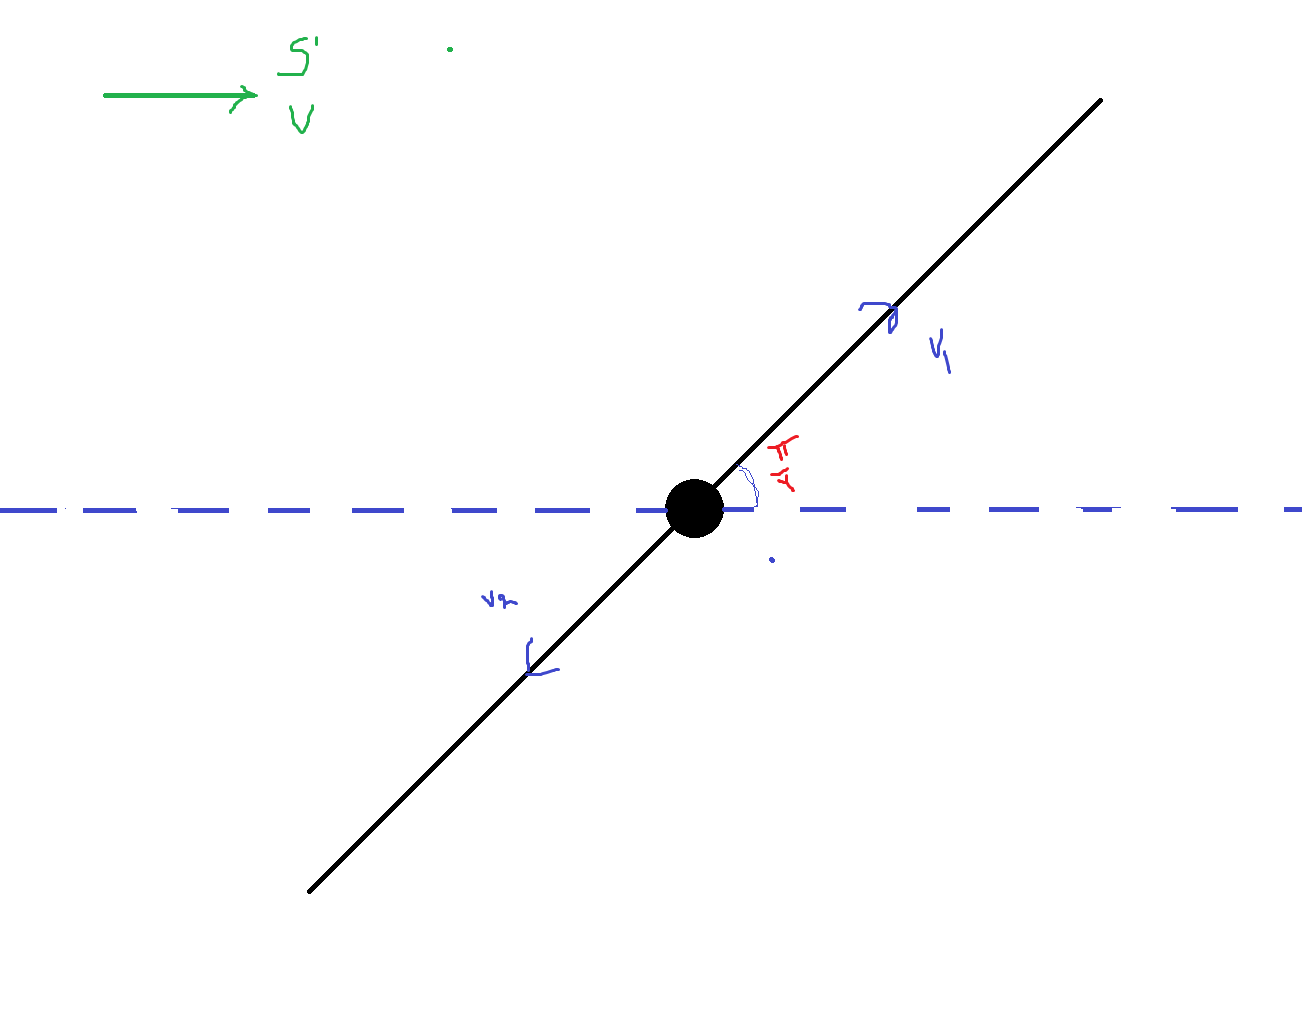
\includegraphics[width=\linewidth]{./lect23/pic1.png}
  \end{center}
  
  
  A mass $m$ is decayed into two equal parts moving in direction $\hat{x}+\hat{y}$ with $v_x, v_y = v$. Frame of reference $S^\prime$ moves with same velocity $V$ in direction $\hat{x}$. Before decay, momentum in $S^\prime$ in direction $\hat{y}$ is $0$. Velocities after decay are
  
  $$v_{1y}^\prime = \frac{v}{\gamma \left( 1 - \frac{v^2}{c^2} \right)} = \frac{v}{1-\frac{v^2}{c^2}}\sqrt{1-\frac{v^2}{c^2}}$$
  $$v_{2y}^\prime = -\frac{v_{2y}}{\gamma \left( 1 - \frac{vv_{2y}}{c^2} \right)} = -\frac{v}{\gamma \left( 1 + \frac{v^2}{c^2} \right)} = \frac{-v}{1+\frac{v^2}{c^2}}\sqrt{1-\frac{v^2}{c^2}}$$
  
  Since momentum before decay is 0, then after decay it must be 0 too. That means that classical momentum expression ($mv$) isn't good anymore.
  
  We need to find new expression for momentum:
  
  \begin{enumerate}
  	\item Same formulation for all inertial frames of references
  	\item Switch between frame of references using Lorentz transformation
  	\item If $v \ll c$, we get Newtonian mechanics.
  \end{enumerate}
  
  Clues:
  
  \begin{enumerate}
  	\item $\gamma = \frac{1}{\sqrt{1 - \frac{v^2}{c^2}}}$
  	\item $\delta y$ is equal for all observers moving in direction $\hat{x}$
  	\item $\Delta\tau$ - proper time is identical for all observers: $\Delta \tau = \Delta t \sqrt{1 - \frac{v^2}{c^2}}$
  \end{enumerate}
  
Based on 2 and 3 we create new quantity $$\frac{\Delta y}{\Delta \tau} = \frac{\Delta y}{\Delta t} \frac{\Delta t}{\Delta \tau} = v_y \frac{1}{\frac{d\tau}{dt}} = v_y = \frac{1}{\sqrt{1 - \frac{v^2}{c^2}}} = \gamma v_y $$.
	
	\paragraph{Relative momentum} acquired from clues:
	$$\vec{p} = \frac{m\vec{v}}{\sqrt{1-\frac{v^2}{c^2}}} = \gamma m \vec{v}$$
	
\subsection{Energy}

$$K = E_k = \left(\parbox{1.5cm}{\centering \scriptsize Work to get particle from v=0 to v=v}\right)$$

Substitute force from Newtonian mechanics ($\vec{F} =\frac{\vec{p}}{t}$):

$$K=W= \int_0^{x_f} \vec{F} \left(dx\hat{x}\right) =  \int_0^{x_f} \frac{d}{dt} \left[ \frac{mv}{\left( 1-\frac{v^2}{c^2} \right)^\frac{1}{2}} \right] dx \stackrel{\parbox{1cm}{\centering \scriptsize switch of integration variable}}{=} \int_0^{t_f} \left[ \frac{m \frac{dv}{dt}}{\left( 1-\frac{v^2}{c^2} \right)^\frac{1}{2}} -\frac{1}{2} \frac{mv\left( \frac{-2v}{c^2} \right) \frac{dv}{dc}}{\left( 1-\frac{v^2}{c^2} \right)^\frac{3}{2}} \right]\frac{dv}{dt}dt$$

$$K = \int_{0}^{t_f} \frac{mv\frac{dv}{dt}}{\left( 1-\frac{v^2}{c^2} \right)^\frac{3}{2}}dt = \int_0^{t_f} \frac{d}{dt} \left[ \frac{mc^2}{\left( 1-\frac{v^2}{c^2} \right)^\frac{1}{2}} \right] dt$$

By substituting $v_0=0$ and $v_f=v$:

$$K = \frac{mc^2}{\left( 1-\frac{v^2}{c^2} \right)^\frac{1}{2}} - mc^2$$

$$K = \gamma mc^2 - mc^2$$

When $ \gamma mc^2$ is total energy of the body and $mc^2$ is rest energy of the body.

$$E{rest} = mc^2$$
$$E = \gamma mc^2$$

\paragraph{Back to Newton} $v \ll c$:

$$\frac{1}{\sqrt{1-\frac{v^2}{c^2}}}= \left(1-\frac{v^2}{c^2}\right)^{\frac{1}{2}} = 1+\frac{v^2}{2c^2}$$
	
	Then 
	
	$$E_k =\left(1+\frac{v^2}{2c^2}\right)mc^2 - mc^2 = \frac{1}{2}mv^2$$ 
	
\paragraph{Exact development of momentum}

$$1 = \frac{1-\frac{v^2}{c^2}}{1-\frac{v^2}{c^2}} = \frac{1}{1-\frac{v^2}{c^2}} - \frac{\frac{v^2}{c^2}}{1-\frac{v^2}{c^2}} = \gamma^2 - \frac{v^2}{c^2}\gamma^2$$

Since LHS is invariant, then RHS is also invariant. $m^2c^4$ is also invariant since both $m$ and $c$ are invariant. By multiplying we get:

$$m^2c^4=m^2c^4\left(\gamma^2 - \frac{v^2}{c^2}\gamma^2\right)$$
$$\left( mc^2\right)^2 = \left( \gamma mc^2\right)^2  - \left( \gamma mvc\right)^2 $$

It looks like another expression:

$$\left( c \Delta \tau\right)^2 = \left( c \Delta t\right)^2 - \left( \Delta \vec{r} \right)^2$$

By using connections between symmetry in time and conservation of energy and also between symmetry in space and conservation of moment we get $\vec{p} = \gamma m \vec{v}$ and $E=\gamma mc^2$ and also following expression:

$$m^2c^4 = E^2 - \left(pc\right)^2$$

Also 

$$E = \sqrt{p^2c^2 - m^2c^4}$$

If $v \ll c$ then $p \ll mc$ and

$$E  \simeq mc^2 + \underbrace{\frac{p^2}{2m}}_{\parbox{1.5cm}{\centering \scriptsize Kinetic enegrgy in Newtonian mechanics}}$$
	
	Opposite, if $p \gg mc$ then
	
	$$E \approx pc$$
	
	For  photon, $m=0$,
	
	$$E = pc$$
And

$$p = \frac{E}{c} = \frac{hf}{c} = \frac{h}{\lambda}$$

